\documentclass[a4paper, 20pt,reqno]{article}
\usepackage[left=2cm,right=2cm,top=2cm,bottom=2cm]{geometry}
\usepackage[T2A]{fontenc}
% \DeclareMathSizes{10}{10}{10}{10}

\usepackage[russian]{babel}
\usepackage{soul}
\usepackage{gensymb}
\usepackage{amsfonts,amsmath,amssymb}
\usepackage{mathrsfs}
\usepackage{graphicx}
\usepackage[normalem]{ulem}
\usepackage[document]{ragged2e}
\usepackage{stmaryrd}
\usepackage{wrapfig}
\usepackage{fancyhdr}
\usepackage{floatflt}
\usepackage{python}
\usepackage{float}
\usepackage{amssymb}
\usepackage[most]{tcolorbox}
\usepackage{indentfirst}
\usepackage{setspace}
\usepackage{scrextend}
\usepackage{listings}
\usepackage{makecell,tabularx}
\usepackage{hyperref}
\usepackage{xcolor}

\newcommand{\mycopyright}{pluttan}
\newcommand{\docopyright}{$\mathfrak{Copyright}\ \mathfrak{\mycopyright} \logo$}
\newcommand{\rub}{{\rm{Р}\kern-.635em\rule[.5ex]{.52em}{.04em}\kern.11em}}

\definecolor{linkcolor}{HTML}{000000} 
\definecolor{urlcolor}{HTML}{0000FF} 

\hypersetup{pdfstartview=FitH,  linkcolor=linkcolor,urlcolor=urlcolor, colorlinks=true}

\definecolor{grey}{RGB}{40, 40, 40}

\renewcommand{\href}[1]{\url{#1}}

\definecolor{codegreen}{rgb}{0,0.6,0}
\definecolor{codegray}{rgb}{0.5,0.5,0.5}
\definecolor{codepurple}{rgb}{0.7,0,0.82}
\definecolor{mermaid}{rgb}{0.5,0.3,1}
\definecolor{backcolour}{rgb}{0.95,0.95,0.92}

\lstdefinestyle{mystyle}{
    backgroundcolor=\color{backcolour},   
    commentstyle=\color{codegreen},
    keywordstyle=\color{mermaid},
    numberstyle=\tiny\color{codegray},
    stringstyle=\color{codepurple},
    basicstyle=\ttfamily\footnotesize,
    breakatwhitespace=false,         
    breaklines=true,                 
    captionpos=b,                    
    keepspaces=true,                 
    numbers=left,                    
    numbersep=5pt,                  
    showspaces=false,                
    showstringspaces=false,
    showtabs=false,                  
    tabsize=2,
  extendedchars=true , % включаем не латиницу 
  escapechar=|, % |«выпадаем» в LATEX|
  frame=tb , % рамка сверху и снизу 
  commentstyle=\itshape , % шрифт для комментариев 
  stringstyle=\bfseries
}

\lstset{style=mystyle}

\lstdefinestyle{CommentStyle}{
    language=XML,
    %numbers=left, numberstyle=\tiny, stepnumber=1, numbersep=5pt,
    commentstyle=\color{red},
	basicstyle=\footnotesize\ttfamily,
	language={[ANSI]C++},
	keywordstyle=\bfseries,
	showstringspaces=false,
	morekeywords={include, printf},
	commentstyle={},
	escapeinside=§§,
	escapebegin=\begin{russian}\commentfont,
	escapeend=\end{russian},
    keywordstyle=\color{blue}\bfseries,
    morekeywords={align,begin},
    extendedchars=\true,
    tabsize=2
}
\lstdefinestyle{myLatexStyle}{
    language=c++,
    %backgroundcolor=\color{grey},
    numbers=left, numberstyle=\tiny, stepnumber=1, numbersep=5pt,
    commentstyle=\color{red},
    keywordstyle=\color{blue}\bfseries,
    morekeywords={align,begin},
    extendedchars=\true,
    tabsize=2
}

\lstdefinestyle{pmyLatexStyle}{
    language=java,
    %backgroundcolor=\color{grey},
    numbers=left, numberstyle=\tiny, stepnumber=1, numbersep=5pt,
    commentstyle=\color{red},
    keywordstyle=\color{blue}\bfseries,
    morekeywords={align,begin},
    extendedchars=\true,
    tabsize=2
}

\definecolor{block-gray}{gray}{0.90} % уровень прозрачности (1 - максимум)
\definecolor{yellow}{HTML}{F0FFFF}
\newtcolorbox{myquote}{colback=block-gray,grow to right by=-10mm,grow to left by=-10mm,boxrule=0pt,boxsep=0pt,breakable} % настройки области с изменённым фоном
\newtcolorbox{myquote2}{colback=yellow,grow to right by=-10mm,grow to left by=-10mm,boxrule=0pt,boxsep=0pt,breakable} % настройки области с изменённым фоном

\setlength{\parindent}{12,5mm}

\newcommand{\logo}{\vcenter{\hbox{
\includegraphics[width=.8em]{/Users/pluttan/Documents/bw2.png}}}}
\onehalfspacing

\pagestyle{fancy}
\renewcommand{\sectionmark}[1]{\markright{#1}}
\fancyhf{} 
\fancyhead[R]{\bfseries\thepage}
\fancyhead[LO]{\docopyright}

\newcommand{\image}[2]{
	\begin{figure}[H]
		\center{\includegraphics[height=#2pt]{../img/#1} }
    \end{figure}
}

\newcommand{\dotitle}[2]{

\thispagestyle{empty}
\sloppy{
  \scriptsize{
    \line(6,0){0}

    \centering \docopyright

    \centering Привет! Меня зовут Андрей, я создаю свою ботву, этот файл малая ее часть. 
    
    \centering Пользоваться и распространять файлы конечно же можно. Если вы нашли ошибку в файле, можете 
    
    \centering исправить ее в исходном коде и подать на слияние или просто написать в issue. 

    \centering {\bf{Так же вы можете купить распечатанную версию данного файла в виде книжки.}
    
    \centering По всем вопросам писать в ВК.}
    
    \centering Приятного бота)

    \line(6,0){300}

    \centering GitHub: \href{https://github.com/pluttan}

    \centering VK: \href{https://vk.com/pluttan}

    \line(6,0){0}
  }}

\begin{figure}[H]
		\center{\includegraphics[height=100pt]{/Users/pluttan/Documents/forMyDocs/qr2.png} }
\end{figure}

\topskip=-200pt
\vspace*{130pt}
\begin{Huge}
  \textbf{
    \begin{center}
        #1
    \end{center}
  }
  {\begin{center} 
        #2
    \end{center}}
\end{Huge}
\vspace*{300pt}
  \begin{flushright}
    Над файлом работали: \\
    \mycopyright
  \end{flushright}
\newpage
\pagestyle{fancy}
\renewcommand{\sectionmark}[1]{\markright{#1}}
\fancyhf{} 
\fancyhead[R]{\bfseries\thepage}
\fancyhead[LO]{\docopyright}
}
\renewcommand{\sectionmark}[1]{\markright{#1}}
\renewcommand{\sectionmark}[1]{\markright{#1}}
% \makeatletter
%      \renewcommand*\l@section{\@dottedtocline{1}{0em}{1.8em}}
%      \renewcommand*\l@subsection{\@dottedtocline{2}{1.5em}{2.0em}}
%      \renewcommand*\l@subsubsection{\@dottedtocline{3}{4.3em}{3.0em}}
% \makeatother
\newcommand{\toc}{
\newpage
\renewcommand{\contentsname}{Оглавление}
\large{\tableofcontents}
\newpage
\large
}


% It's XeLaTeX, if you can't compile comment this line 
\usepackage{fontspec}\setmainfont{Times New Roman} 

\renewcommand{\dotitle}[2]{

\thispagestyle{empty}
\begin{minipage}[l]{300pt}
  \vspace*{25pt}
  \sloppy{
  \scriptsize{
    \line(6,0){0}

    \centering \docopyright

    \centering Привет! Это Трубусы и Уточки, мы создаем свою ботву, этот файл малая ее часть. 
    
    \centering Пользоваться и распространять файлы конечно же можно. Если вы нашли ошибку в файле, можете 
    
    \centering исправить ее в исходном коде и подать на слияние или просто написать в issue. 

    \centering \textbf{Так же вы можете купить распечатанную версию данного файла в виде книжки.}
    
    \centering \textbf{По всем вопросам писать в ВК.}
    
    \centering Приятного бота)

    \line(6,0){300}

    \centering GitHub: \href{https://github.com/pluttan}

    \centering VK: \href{https://vk.com/pluttan}

    \centering VK: \href{https://vk.com/f_i_i_x_i_i}

    \line(6,0){0}}
}
\end{minipage}
\begin{minipage}[r]{150pt}
  \raggedright
\includegraphics[height=150pt]{/Users/pluttan/Documents/forMyDocs/qr1.png}
\end{minipage}


\topskip=-250pt
\vspace*{170pt}
\begin{Huge}
  \textbf{
    \begin{center}
        #1
    \end{center}
  }
  {\begin{center} 
        #2
    \end{center}}
\end{Huge}
\vspace*{250pt}
  \begin{flushright}
    Над файлом работали: \\
    \mycopyright
  \end{flushright}
% \newpage
\pagestyle{fancy}
\renewcommand{\sectionmark}[1]{\markright{#1}}
\fancyhf{} 
\fancyhead[R]{\bfseries\thepage}
\fancyhead[LO]{\docopyright}
}
\renewcommand{\mycopyright}{pluttan \& fiixii}

\begin{document}
\tikz[remember picture,overlay] \node[opacity=0.1,inner sep=0pt] at (current page.center){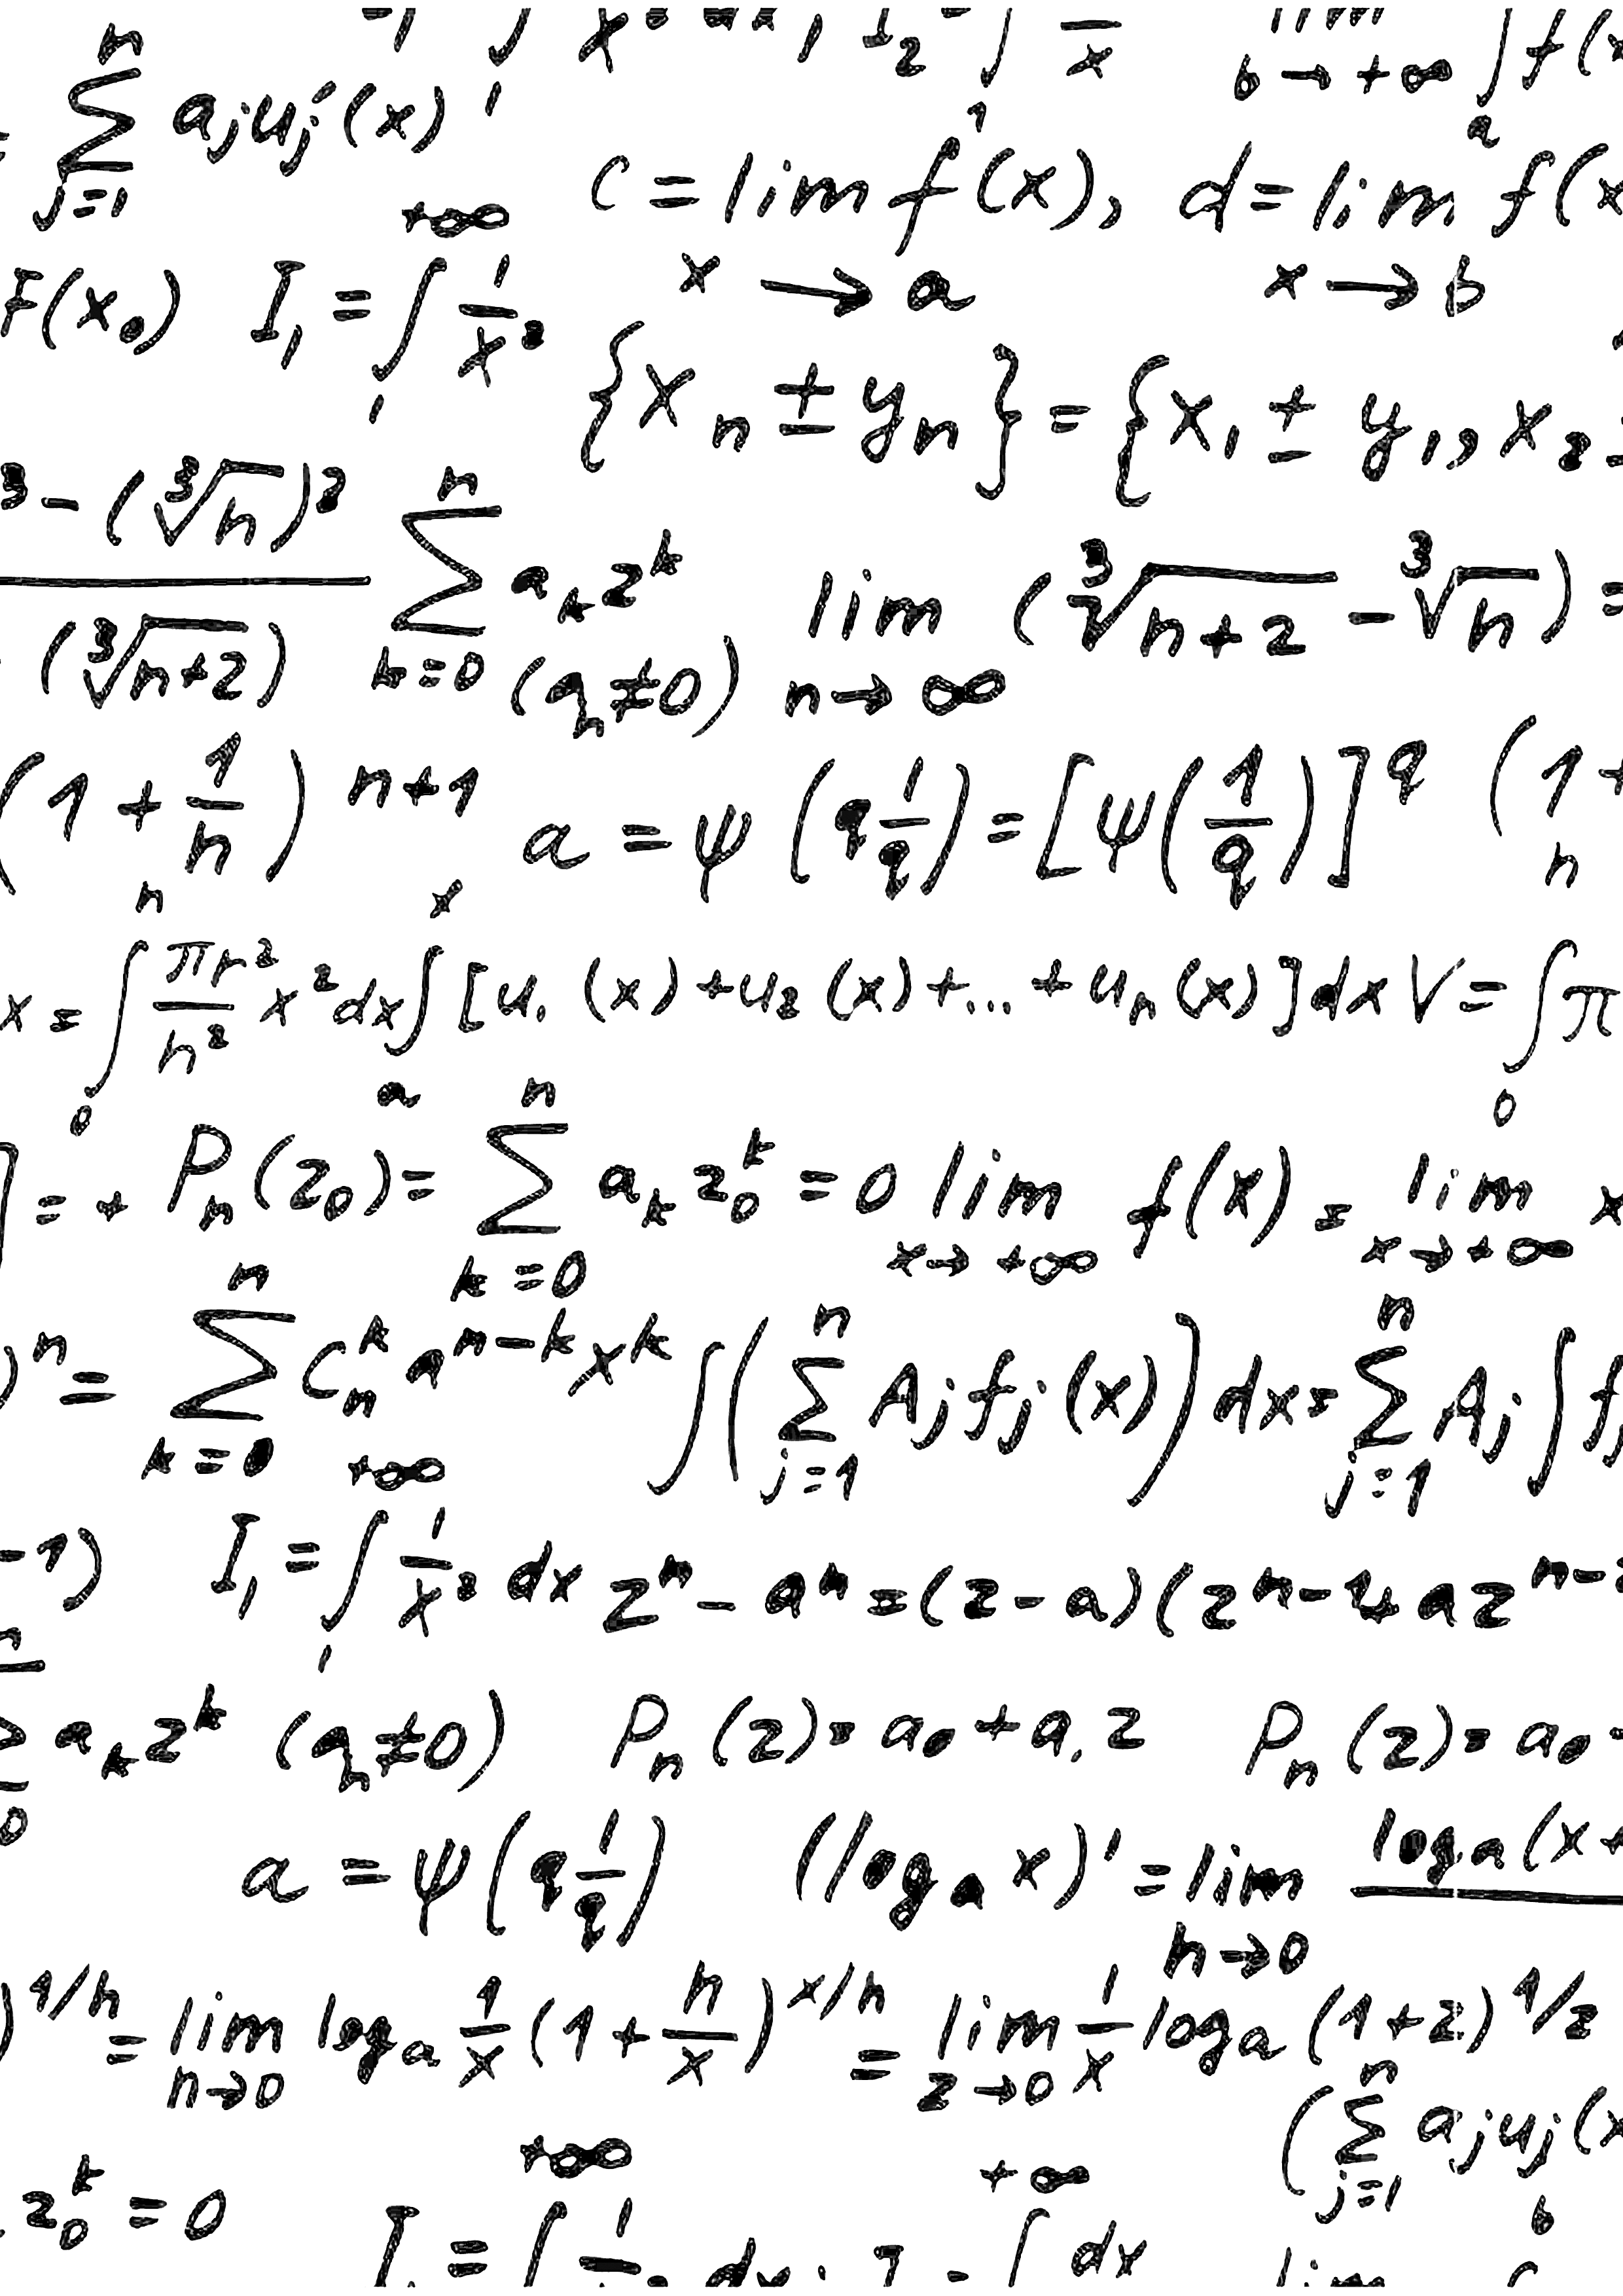
\includegraphics[width=\paperwidth,height=\paperheight]{../img/bg100.png}};
\dotitle{Подготовка к РК2}{Математический анализ}
% //SECTION Определения
\section{Определения}

% //SUBSECTION 1. Сформулируйте определение наклонной асимптоты.
\subsection{Сформулируйте определение наклонной асимптоты.}

Пусть функция $y = f(x)$ определена при x > x0 (x < x0). Если функция при $x \rightarrow +\infty (-\infty)$ представима в виде: f(x) = Ax + B + o(1), то прямую y = Ax + B называют наклонной правой (левой) асимптотой графика функции f(x).


% //!SUBSECTION 

% //SUBSECTION 2. Сформулируйте определение производной функции в точке.
\subsection{Сформулируйте определение производной функции в точке.}

Пусть $f(x)$ определена в окрестности точки $x_0$ и пусть $\Delta x \ne 0$ таково, что $x_0+\Delta x$ принадлежит указанной окрестности. Если $\exists$ конечный предел $\lim\limits_{\Delta x \to 0}\frac{f(x_0+\Delta x) - f(x_0)}{\Delta x}$, то он называется производной $f(x)$ в точке $x_0$.

% //!SUBSECTION 

% //SUBSECTION 3. Сформулируйте определение односторонней производной функции.
\subsection{Сформулируйте определение односторонней производной функции.}

Если $f(x)$ определена в правосторонней (левосторонней) окрестности точки $x_0$, т.е. на полуинтервале $[x_0,x_0+\eta)$ $(x_0,x_0+\eta])$, $\eta > 0$ и если $\exists \lim\limits_{\Delta x \to 0+(0-)}\frac{f(x_0+\Delta x) - f(x_0)}{\Delta x}$, то этот предел называется правой (левой) производной функции $f(x)$ в $x_0$.

% //!SUBSECTION 


% //SUBSECTION 4. Сформулируйте определение производной n-го порядка.
\subsection{Сформулируйте определение производной n-го порядка.}

Производная $n$-ого порядка от функции $y = f(x)$, есть производная от производной $n-1$ порядка $y^{(n)} = (f^{n-1}(x))$.


% //!SUBSECTION 

% //SUBSECTION 5. Сформулируйте определение дифференцируемой функции в точке.
\subsection{Сформулируйте определение дифференцируемой функции в точке.}

Пусть функция $y = f(x)$ определена в некоторой окрестности точки $x_0$. Функция $f(x)$ называется дифференцируемой в точке $x_0$, если ее приращение $\Delta y$ в точке $x_0$ представимо в следующем виде: $\Delta y = A\Delta x \ne \alpha(\Delta x)\Delta x$, где $A = f'(x_0)$ и $\lim\limits_{\Delta x \to 0}\alpha (\Delta x) = 0$.

% //!SUBSECTION 


% //SUBSECTION 6. Сформулируйте определение дифференциала первого порядка. 
\subsection{Сформулируйте определение дифференциала первого порядка.}

Линейная от $\Delta x$ функция $A \Delta x (A = f'(x))$ называется дифференциалом функции $f(x)$ 1-ого порядка.

% //!SUBSECTION 


% //SUBSECTION 7. Сформулируйте определение дифференциала n-го порядка.
\subsection{Сформулируйте определение дифференциала n-го порядка.}

Дифференциал $n$-ого порядка называется дифференциал от дифференциала $n - 1$ порядка $\partial^ny = \partial(\partial^{n-1}y) = f^{(n)}(x)\partial x^n$

% //!SUBSECTION 

  
% //SUBSECTION 8. Сформулируйте определение возрастающей функции.
\subsection{Сформулируйте определение возрастающей функции.}

Функция $f(x)$ называется возрастающей на интервале $(a, b)$, если $\forall x_1, x_2 \in (a, b):$ $f(x_2)>f(x_1)$.

% //!SUBSECTION 


% //SUBSECTION 9. Сформулируйте определение невозрастающей функции.
\subsection{Сформулируйте определение невозрастающей функции.}

Функция $f(x)$ называется невозрастающей на интервале $(a, b)$, если $\forall x_1, x_2 \in (a, b):$ $f(x_2) \leqslant f(x_1)$.

% //!SUBSECTION 

% //SUBSECTION 10. Сформулируйте определение убывающей функции.
\subsection{Сформулируйте определение убывающей функции.}

Функция $f(x)$ называется убывающей на интервале $(a, b)$, если $\forall x_1, x_2 \in (a, b):$ $f(x_2)<f(x_1)$.

% //!SUBSECTION 


% //SUBSECTION 11. Сформулируйте определение неубывающей функции.
\subsection{Сформулируйте определение неубывающей функции.}

Функция $f(x)$ называется неубывающей на интервале $(a, b)$, если $\forall x_1, x_2 \in (a, b):$ $f(x_2) \geqslant f(x_1)$.

% //!SUBSECTION 


% //SUBSECTION 12. Сформулируйте определение монотонной функции.
\subsection{Сформулируйте определение монотонной функции.}

Функция $f(x)$ называется монотонной, если она невозрастающая или неубывающая.

% //!SUBSECTION 


% //SUBSECTION 13. Сформулируйте определение строго монотонной функции.
\subsection{Сформулируйте определение строго монотонной функции.}

Функция $f(x)$ называется строго монотонной, если она возрастающая или убывающая.

% //!SUBSECTION 


% //SUBSECTION 14. Сформулируйте определение локального минимума.
\subsection{Сформулируйте определение локального минимума.}

Точка $x_0$ называется точкой локального минимума функции $f(x)$, если $\exists U_{\delta}(x_0)$, такая что $\forall x \in U_{\delta}(x_0)$: $f(x_0) \leqslant f(x)$

% //!SUBSECTION 


% //SUBSECTION 15. Сформулируйте определение строгого локального минимума.
\subsection{Сформулируйте определение строгого локального минимума.}

Точка $x_0$ называется точкой строгого локального минимума функции $f(x)$, если $\exists \overset{\circ}{U}_{\delta}(x_0)$, такая что $\forall x \in \overset{\circ}{U}_{\delta}(x_0)$: $f(x_0) < f(x)$

% //!SUBSECTION 


% //SUBSECTION 16. Сформулируйте определение локального максимума.
\subsection{Сформулируйте определение локального максимума.}

Точка $x_0$ называется точкой локального максимума функции $f(x)$, если $\exists U_f(x_0)$, такая что $\forall x \in U_f(x_0)$: $f(x_0) \geqslant f(x)$

% //!SUBSECTION 


% //SUBSECTION 17. Сформулируйте определение строгого локального максимума.
\subsection{Сформулируйте определение строгого локального максимума.}

Точка $x_0$ называется точкой строгого локального минимума функции $f(x)$, если $\exists \overset{\circ}{U}_f(x_0)$, такая что $\forall x \in \overset{\circ}{U}_f(x_0)$: $f(x_0) < f(x)$

% //!SUBSECTION 


% //SUBSECTION 18. Сформулируйте определение экстремума. 
\subsection{Сформулируйте определение экстремума.}

Точками локального экстремума называются точки локального максимума и строгого локального максимума, локального минимума и строгого локального минимума.

% //!SUBSECTION 


% //SUBSECTION 19. Сформулируйте определение строгого экстремума.
\subsection{Сформулируйте определение строгого экстремума.}

Точками строгого локального экстремума называются точки строгого локального максимума и минимума.

% //!SUBSECTION 


% //SUBSECTION 20. Сформулируйте определение стационарной точки.
\subsection{Сформулируйте определение стационарной точки.}

Точки, в которых производная функции равна 0, называются стандартными.

% //!SUBSECTION 


% //SUBSECTION 21. Сформулируйте определение критической точки.
\subsection{Сформулируйте определение критической точки.}

Точки, в которых производная функции равна 0 или не существует, называются критическими точками функции.

% //!SUBSECTION 


% //SUBSECTION 22. Сформулируйте определение выпуклости функции на промежутке.
\subsection{Сформулируйте определение выпуклости функции на промежутке.}

Пусть функция $f(x)$ определена на интервале $(a, b)$. Говорят, что $f(x)$ является выпуклой вверх(вниз) на этом интервале, если для $\forall$ касательной к графику этой функции каждая точка касательной, отличная от точки касания, лежит выше(ниже) точки графика функции с той же абсциссой.

% //!SUBSECTION 


% //SUBSECTION 23. Сформулируйте определение точки перегиба графика функции.
\subsection{Сформулируйте определение точки перегиба графика функции.}

Точка $x_0 \in (a,b)$ называется точкой перегиба $f(x)$, если эта функция непрерывна в точке $x_0$ и если $\exists \delta > 0$ такое, что направления выпуклостей $f(x)$ на интервалах $(x_0-\delta; x_0)$ и $(x_0; x_0+\delta)$ различны.

% //!SUBSECTION 

% //!SECTION


% //SECTION Формулировки теорем
% \newpage
\section{Формулировки теорем}
% //SUBSECTION 1. Сформулируйте необходимое и достаточное условие наличия наклонной асимптоты [10 ].
\subsection{Сформулируйте необходимое и достаточное условие наличия наклонной асимптоты.}

Пусть функция $f(x)$ определена при $x > x_0 (x < x_0)$. Прямая $y = Ax + B$ тогда и только является правой (левой) асимптотой графика данной функции, когда: 

$\exists \lim\limits_{x \to +\infty (- \infty)}\frac{f(x)}{x} = A$,

$\exists \lim\limits_{x \to +\infty (- \infty)} (f(x)-Ax) = B$

% //!SUBSECTION 

% //SUBSECTION 2. Сформулируйте необходимое и достаточное условие дифференцируемости функции в точке [11 ].
\subsection{Сформулируйте необходимое и достаточное условие дифференцируемости функции в точке.}

Функция $f(x)$ дифференцируема в некоторой точке $x_0$ тогда и только тогда, когда существует производная $f'(x_0)$ в этой точке.

% //!SUBSECTION 

% //SUBSECTION 3. Сформулируйте теорему о связи дифференцируемости и непрерывности функции. [11 ]
\subsection{Сформулируйте теорему о связи дифференцируемости и непрерывности функции.}

Если функция дифференцируема в некоторой точке, то она непрерывна в этой точке.

% //!SUBSECTION 

% //SUBSECTION 4. Сформулируйте теорему о производной произведения. [11 ]
\subsection{Сформулируйте теорему о производной произведения.}

Пусть функции $f(x)$ и $g(x)$ дифференцируемы в точке $x_0$. Тогда в этой точке дифференцируема также функция $f(x)g(x)$, причём $(f(x)g(x))' = f'(x)g(x)+f(x)g'(x)$

% //!SUBSECTION 

% //SUBSECTION 5. Сформулируйте теорему о производной частного. [11 ]
\subsection{Сформулируйте теорему о производной частного.}

Пусть функции $f(x)$ и $g(x)$ дифференцируемы в точке $x_0$ и $(g(x) \ne 0)$. Тогда в этой точке дифференцируема также функция $\frac{f(x)}{g(x)}$, причём $\frac{f'(x)g(x)-f(x)g'(x)}{(g(x))^2}$

% //!SUBSECTION 

% //SUBSECTION 6. Сформулируйте свойство инвариантности формы записи дифференциала первого порядка [12 ].
\subsection{Сформулируйте свойство инвариантности формы записи дифференциала первого порядка.}

Дифференциал функции $y = f(u)$ не зависит от того, является ли $u$ независимой переменной или функцией от другой независимой переменной.

% //!SUBSECTION 

% //SUBSECTION 7. Сформулируйте теорему Ферма. [13 ]
\subsection{Сформулируйте теорему Ферма.}

Пусть функция $f(x)$ определена на промежутке $I$ и в некоторой внутренней точке $x_0$ этого промежутка принимает наибольшее (или наименьшее) значение на этом промежутке. Тогда, если существует производная $f'(x_0)$, то она равна нулю.

% //!SUBSECTION 

% //SUBSECTION 8. Сформулируйте теорему Ролля. [13 ] 
\subsection{Сформулируйте теорему Ролля.}

Пусть функция $f(x)$:
\begin{itemize}
    \item непрерывна на отрезке $[a,b]$;
    \item дифференцируема на интервале $(a,b)$;
    \item $f(a) = f(b)$. 
\end{itemize}

Тогда на интервале $(a,b)$ найдётся точка $c$ такая, что $f'(c) = 0$.

% //!SUBSECTION 

% //SUBSECTION 9. Сформулируйте теорему Лагранжа. [13 ] 
\subsection{Сформулируйте теорему Лагранжа.}

Пусть функция $f(x)$:
\begin{itemize}
    \item непрерывна на отрезке $[a,b]$;
    \item дифференцируема на интервале $(a,b)$;
\end{itemize} 

Тогда на этом интервале существует точка $c$ такая, что $f(b) − f(a) =f'(c)(b − a)$.

% //!SUBSECTION 

% //SUBSECTION 10. Сформулируйте теорему Коши. [13 ]
\subsection{Сформулируйте теорему Коши.}

Пусть функции $f(x)$ и $g(x)$:
\begin{itemize}
    \item непрерывны на отрезке $[a,b]$;
    \item дифференцируемы на интервале $(a,b)$;
    \item $g'(x)$ отлична от нуля в каждой точке этого интервала. 
\end{itemize}

Тогда на интервале $(a, b)$ найдется точка $c$ такая, что $\frac{f(b)-f(a)}{g(b)-g(a)} = \frac{f'(c)}{g'(c)}$.

% //!SUBSECTION 
\vspace*{45pt}
% //!SECTION

\begin{myquote}
Заметочка: на РК2 очень часто встречаются формулы понижения степени

$$\sin^2\alpha = \frac{1 - \cos2\alpha}{2}$$
$$\cos^2\alpha = \frac{1 + \cos2\alpha}{2}$$
\end{myquote}


\newpage
\let\clearpage\relax

\end{document}


